% *======================================================================*
%  Cactus Thorn template for ThornGuide documentation
%  Author: Ian Kelley
%  Date: Sun Jun 02, 2002
%  $Header$                                                             
%  Thorn documentation in the latex file doc/documentation.tex 
%  will be included in ThornGuides built with the Cactus make system.
%  The scripts employed by the make system automatically include 
%  pages about variables, parameters and scheduling parsed from the 
%  relevent thorn CCL files.
%  
%  This template contains guidelines which help to assure that your     
%  documentation will be correctly added to ThornGuides. More 
%  information is available in the Cactus UsersGuide.
%                                                    
%  Guidelines:
%   - Do not change anything before the line
%       % BEGIN CACTUS THORNGUIDE",
%     except for filling in the title, author, date etc. fields.
%        - Each of these fields should only be on ONE line.
%        - Author names should be sparated with a \\ or a comma
%   - You can define your own macros are OK, but they must appear after
%     the BEGIN CACTUS THORNGUIDE line, and must not redefine standard 
%     latex commands.
%   - To avoid name clashes with other thorns, 'labels', 'citations', 
%     'references', and 'image' names should conform to the following 
%     convention:          
%       ARRANGEMENT_THORN_LABEL
%     For example, an image wave.eps in the arrangement CactusWave and 
%     thorn WaveToyC should be renamed to CactusWave_WaveToyC_wave.eps
%   - Graphics should only be included using the graphix package. 
%     More specifically, with the "includegraphics" command. Do
%     not specify any graphic file extensions in your .tex file. This 
%     will allow us (later) to create a PDF version of the ThornGuide
%     via pdflatex. |
%   - References should be included with the latex "bibitem" command. 
%   - use \begin{abstract}...\end{abstract} instead of \abstract{...}
%   - For the benefit of our Perl scripts, and for future extensions, 
%     please use simple latex.     
%
% *======================================================================* 
% 
% Example of including a graphic image:
%    \begin{figure}[ht]
% 	\begin{center}
%    	   \includegraphics[width=6cm]{MyArrangement_MyThorn_MyFigure}
% 	\end{center}
% 	\caption{Illustration of this and that}
% 	\label{MyArrangement_MyThorn_MyLabel}
%    \end{figure}
%
% Example of using a label:
%   \label{MyArrangement_MyThorn_MyLabel}
%
% Example of a citation:
%    \cite{MyArrangement_MyThorn_Author99}
%
% Example of including a reference
%   \bibitem{MyArrangement_MyThorn_Author99}
%   {J. Author, {\em The Title of the Book, Journal, or periodical}, 1 (1999), 
%   1--16. {\tt http://www.nowhere.com/}}
%
% *======================================================================* 

% If you are using CVS use this line to give version information
% $Header$

\documentclass{article}

% Use the Cactus ThornGuide style file
% (Automatically used from Cactus distribution, if you have a 
%  thorn without the Cactus Flesh download this from the Cactus
%  homepage at www.cactuscode.org)
\usepackage{../../../../doc/latex/cactus}

\begin{document}

% The author of the documentation
\author{Cactus Maintainers \textless\code{cactusmaint@cactuscode.org}\textgreater}

% The title of the document (not necessarily the name of the Thorn)
\title{Coordinate Base Thorn}

% the date your document was last changed:
\date{$ $Date$ $}

\maketitle

% Do not delete next line
% START CACTUS THORNGUIDE

% Add all definitions used in this documentation here:
\def\WRAGH{CCTK\_WRAGH}
\def\beforetable{\\[1mm]}

\hyphenation{Coord}

% Add an abstract for this thorn's documentation
\begin{abstract}
CoordBase provides a mechanism for registering coordinate systems, and
maintaining a database of coordinate systems and their coordinates,
using key-value tables.

CoordBase also provides a way for specifying the extent of the
simulation domain that is independent of the actual coordinate and
symmetry thorns, and for specifying the discretisation of the boundary
that is independent of the actual boundary thorns.
\end{abstract}


\section{Introduction}

Many applications which use Cactus will want to make use of coordinate
systems.  The CoordBase thorn provides a method of registering
coordinate systems and their properties.  Thorns which implement
coordinate systems will register the systems they provide with
CoordBase.  Since coordinate systems are composed of a collection of
coordinates, the coordinates which comprise the systems are registered
with CoordBase as well.  The data describing coordinate systems are
held on Cactus key-value tables.  A schema for the format of these
tables is provided in section
\ref{CactusBase_CoordBase_coordinate_schema}.  Developers are free to
compose and use their own schema, but are encouraged to use the one
detailed here, as this will be the standard for all of the core Cactus
thorns.

CoordBase specifies an extensible set of coordinate properties.  The
use of key-value tables to hold these properties makes CoordBase
flexible and configurable.  The coordinate values themselves can be
specified in a number of ways, depending on the nature of the
coordinate system.  This way symmetries of the coordinates on the
computational grid can be exploited to minimize memory consumption.
Via a function call, one can easily ascertain what coordinate system is
associated with any given grid variable, which is convenient for e.g.\
I/O.  A method of registering default coordinates for all grid
variables of a certain dimension makes it simple to specify which
coordinate systems should be associated with which grid variables.

The coordinate infrastructure provided by CoordBase will work
seamlessly with AMR and multi-model codes.

%extensible database of coordinate systems, coordinates, and their
%properties

Thorns which provide coordinates will inherit from CoordBase, and
register both the coordinate systems they provide, and the default
coordinate systems for the appropriate dimension of grid variables.
In addition, one can associate a coordinate with any Cactus grid
variable, within a thorn's interface.ccl.
Coordinate systems specified in the interface.ccl override defaults
for the dimension.

The coordinate functions in the Cactus flesh are deprecated with the
introduction of this thorn.  Please use the functions provided here in
preference to those in the flesh.


\section{Coordinate system symmetries}

Since computations performed with Cactus are done on a discrete
lattice, only a discrete set of coordinate values are used for any
coordinate system.  The symmetries of how the coordinate values vary
on the grid points make coordinates fall into three types:
\emph{uniform}, \emph{nonuniform}, and \emph{warped}.  (At least these
are the three cases that the CoordBase schema considers.)  A uniform
coordinate varies from each of its neighbors by a constant.  i.e.\ its
value can be determined from the index of the grid point from simply
an origin and constant `delta'.  A nonuniform coordinate has a
spatially varying `delta'.  For both uniform and nonuniform
coordinates, the coordinate values do not vary along the other
directions of the grid.  (e.g.\ the $x$ coordinate will be the same
regardless of the `j' index of the grid point.)  Thus one could
completely determine the coordinate values of a 3D system of
nonuniform coordinates by providing three 1D arrays.  This later
assumption is relaxed for a warped coordinate; a warped coordinate
will vary across the entire grid.  Recall that `coordinate lines'
(lines of constant coordinate value) cannot cross (because one n-tuple
of coordinate values would specify muliple points in space), so this
places a `bound' of sorts on the possible `warping' of the
coordinates.

The type of a coordinate system will be the same as that of its
coordinates.  If there are different types of coordinates within the
same system, then the coordinate system is \emph{mixed}.  Note that a
warped coordinate system is the most general possible, so any
coordinate system could be regarded as warped if one wishes.

\subsection{Specifying coordinate values}

As mentioned above, for a uniform coordinate system, it is sufficient
to specify the origin and spacing for a uniform coordinate.  One may
also specify a grid variable to hold the coordinate values, if
desired.  See section \ref{CactusBase_CoordBase_coordinate_schema}.  A
nonuniform coordinate can be specified with a 1D grid variable, if
desired, or an nD variable.  A warped coordinate system will always
need a nD grid variable.  FMR and AMR will need an nD grid
variable to specify the coordinate values.  A mixed coordinate system
can use some combination of the above, or simply an nD grid variable.


\section{Coordinate Thorns}

Generally coordinate thorns will allow the declaration of default
coordinate systems for a dimension to be controled by parameters.

If a thorn attempts to register a default for a dimension which
already has a default registered, a level 1 warning will result, and
the default will be overwritten with the new default.  Since the order
of execution of the registration calls will in general not be
specified, one must be careful when activating more than one coordinate thorn.

Coordinate systems and defaults can be changed at any time throughout
a run, as can coordinate properties.
In general these are set at \WRAGH\ and CCTK\_BASEGRID, respectively.

The coordinate thorns are responsible for filling out the portions of
the coordinate and coordinate system tables that are not written by
the registration routines.  See sections
\ref{CactusBase_CoordBase_system_tables} and
\ref{CactusBase_CoordBase_coord_tables}.

\section{Application thorns}

Application thorns should check at CCTK\_PARAMCHECK to see if the correct
coordinate system is being used for each relevant grid variable.
While the old flesh API is still being used you may want to make this
merely a warning.
Use Coord\_GroupSystem() to find the coordinate system for groups (see
section \ref{CactusBase_CoordBase_APIs}).


\section{Coordinate APIs}
\label{CactusBase_CoordBase_APIs}

\begin{verbatim}
CCTK_INT systemhandle = Coord_SystemRegister(CCTK_POINTER_TO_CONST GH,
                                             CCTK_INT dim, 
                                             CCTK_STRING systemname)
\end{verbatim}
registers a coordinate system, along with its
dimension, with the CoordBase thorn.  This will create a coordinate
system table, and return the handle of the table for success, or a
negative error code upon error.  The possible errors are:\beforetable
\begin{tabular}{ll}
COORDERROR\_INVALIDDIM   & invalid dimension passed in\\
COORDERROR\_INVALIDNAME  & invalid name passed in\\
COORDERROR\_TABLEERROR   & error from key-value or hash tables in flesh\\
COORDERROR\_SYSTEMEXISTS & coordinate system of this name already exists\\
\end{tabular}
\\These error codes are defined in CoordBase.h.  CoordBase holds the
table handles on a GH extension, under the name ``CoordBase''.

\begin{verbatim}
CCTK_INT systemhandle = Coord_SystemHandle(CCTK_POINTER_TO_CONST GH,
                                           CCTK_STRING systemname)
\end{verbatim}
returns the handle for a given coordinate system, or 
negative on error:\beforetable
\begin{tabular}{ll}
   COORDERROR\_TABLEERROR &  error from hash table\\
   COORDERROR\_NOSYSTEM   &  no coordinate system of this name is registered\\
\end{tabular}

\begin{verbatim}
CCTK_INT coordhandle = Coord_CoordRegister(CCTK_POINTER_TO_CONST GH, 
                                           CCTK_INT systemhandle, 
                                           CCTK_INT direction,
                                           CCTK_STRING coordname)
\end{verbatim}
registers a coordinate within a coordinate system, in the specified
`direction'.  (Direction in this context means the index in the
coordinate basis, which ranges from 1 to the dimension of the system.)
Coord\_CoordRegister() returns the coordinate handle, or negative for an 
error:\beforetable
\begin{tabular}{ll}
COORDERROR\_INVALIDDIM       & invalid `direction'\\
COORDERROR\_INVALIDHANDLE    & invalid handle passed in / coordinate system
                               does not exist\\
COORDERROR\_TABLEERROR       & error from hash or key-value tables in flesh\\
COORDERROR\_COORDINATEEXISTS & coordinate already exists for this `direction'\\
COORDERROR\_DUPLICATENAME    & coordinate of this name already exists in this
                               system\\
\end{tabular}

\begin{verbatim}
CCTK_INT coordhandle = Coord_CoordHandle(CCTK_POINTER_TO_CONST GH,
                                         CCTK_STRING coordname,
                                         CCTK_STRING systemname)
\end{verbatim}
returns the coordinate handle for a given coordinatate in a coordinate system,
or negative on error:\beforetable
\begin{tabular}{ll}
COORDERROR\_NOSYSTEM    & no coordinate system of this name is registered\\
COORDERROR\_TABLEERROR  & error from hash table\\
COORDERROR\_NOSUCHCOORD & no coordinate of the name is registered for this 
                         system\\
\end{tabular}

\begin{verbatim}
int systemhandle = Coord_GroupSystem(const cGH *GH, 
                                     const char *groupname)
\end{verbatim}
returns the handle for the coordinate system associated with a group of grid 
variables, or negative on error.
This can either be the default for coordinate systems of this
dimension, or the coordinate system that is specified in the
interface.ccl.  Coordinate systems specified in interface.ccl will
override any defaults.  The possible error codes are:\beforetable
\begin{tabular}{ll}
COORDERROR\_INVALIDGROUPNAME & no such group exists\\
COORDERROR\_NOCOORDSYS       & no coordinate system is associated with the
                               group
\end{tabular}

\begin{verbatim}
CCTK_INT systemhandle = Coord_SetDefaultSystem(CCTK_POINTER_TO_CONST GH,
                                               CCTK_STRING systemname)
\end{verbatim}
sets this coordinate system to be the default for grid variables of
the same dimension.  It returns the handle of the system, or negative
for errors:\beforetable
\begin{tabular}{ll}
COORDERROR\_INVALIDNAME   & no coordinate system of this name has been 
			    registered\\
COORDERROR\_NODIMENSION   & coordinate system does not have a valid dimension\\
COORDERROR\_DEFAULTEXISTS & grid variables of this dimension already have a \\
                          & default coordinate system registered\\
\end{tabular}
\\There can be a default coordinate system for each grid dimension.  The
default system will apply for each grid variable of that dimension,
unless it is overridden.

\begin{verbatim}
CCTK_INT systemhandle = Coord_GetDefaultSystem(CCTK_POINTER_TO_CONST GH,
                                               CCTK_INT dim)
\end{verbatim}
gets the default coordinate system for grid variables of dimension {\tt dim}
(ranging from 1 to the maximum number of dimensions registered).
It returns the handle of the system, or negative for errors:\beforetable
\begin{tabular}{ll}
COORDERROR\_INVALIDDIM   & given dimension is invalid\\
COORDERROR\_NOSYSTEM     & given dimension does not have a default coordinate 
                           system associated
\end{tabular}


\section{Coordinate Schema}
\label{CactusBase_CoordBase_coordinate_schema}

\subsection{Coordinate System Tables}
\label{CactusBase_CoordBase_system_tables}

Associated with each coordinate system is a table, which should have the
following entries:\beforetable
\begin{tabular}{|l|l|l|}
\hline
\textbf{key} & \textbf{data type} & \textbf{value}\\
\hline
NAME        & CCTK\_STRING & \code{Cart3d|Spher3d|....}\\
DIMENSION   & CCTK\_INT    & \code{1,2,3,...}\\
TYPE        & CCTK\_STRING & \code{uniform|nonuniform|warped|mixed}\\
COORDINATES & CCTK\_INT array & \verb|<coord1>,...<coord_dimension>|\\
\hline
\end{tabular}
\\The values for the coordinates array are the handles for the
coordinate tables (see section
\ref{CactusBase_CoordBase_coord_tables}).  The NAME and DIMENSION
fields are filled out when Coord\_SystemRegister() is called.  The
COORDINATES field is filled out by Coord\_CoordRegister().  It is left
for the coordinate thorn to fill out the TYPE field.

\subsection{Coordinate Tables}
\label{CactusBase_CoordBase_coord_tables}

Associated with each coordinate of each coordinate system is another
table, which should have the following entries:\beforetable
\begin{tabular}{|l|l|l|}
\hline
\textbf{key} & \textbf{data type} & \textbf{values}\\
\hline
SYSTEM        & CCTK\_INT    & \verb|<handle>|\\
NAME          & CCTK\_STRING & \code{x}\\
DIRECTION     & CCTK\_INT    & \code{2}\\
PHYSICALMIN   & CCTK\_INT    & \code{0}\\
COMPMIN       & CCTK\_REAL   & \\
PHYSICALMAX   & CCTK\_INT    & \\
COMPMAX       & CCTK\_REAL   & \\
TYPE          & CCTK\_STRING & \verb/uniform|non-uniform|warped/\\
TIMEDEPENDENT & CCTK\_INT    & \verb/<yes (1)|no (0)>/\\
DATATYPE      & CCTK\_STRING & \\
GAINDEX       & CCTK\_INT    & \\
\hline
DELTA\footnotemark %{only for type=uniform}
              & CCTK\_REAL   & \code{147.372e16}\\
\hline
\end{tabular}
\footnotetext{only for type=\code{uniform}} 
\\
Coord\_CoordRegister() fills out the SYSTEM, NAME, and DIRECTION
fields, and the COORDINATES field of the system table.  The remaining
fields are the responsibility of the coordinate thorn.

% Each of these fields should be explained...  
% Though most are pretty self-explanatory.


\section{Specifying coordinate systems in the interface.ccl}

Coordinate systems associated with grid variable groups can be
specified in the group's tags table, using the key \code{COORDSYSTEM}.
Below is a grid array which could represent a vector field on a
2-sphere.
\begin{verbatim}
CCTK_REAL SphericalVectorField TYPE=ARRAY DIM=2 TAGS='COORDSYSTEM="sphere2d" TENSORTYPE="vector"'
{
  field_theta, field_phi
}
\end{verbatim}
Even though another thorn has set a default for all 2D grid variables
to something else, Coord\_GroupSystem() will always return the handle
for sphere2d when called on this group.


\section{Specifying the extent of the physical domain}
\label{CactusBase:CoordBase:domain}

CoordBase provides a way for specifying the extent of the simulation
domain that is independent of the actual coordinate and symmetry
thorns.  This is necessary because the size of the physical domain is
not necessarily the same as the size of the computational grid, which
is usually enlarged by symmetry zones and/or boundary zones.

The physical domain is characterised by the location of its lower and
upper boundary and by its grid spacing.  These quantities are related
to the extent and the number of grid cells that span the domain.  The
relation between the size of the domain and the size of the
computational grid is defined in section
{\ref{CactusBase:CoordBase:domain}} below.  The domain extent as
defined in this section is the continuum extent and is independent of
the actual discretisation.  This makes it possible to adapt the same
domain specification for different resolutions by changing only a
single parameter.

The domain is specified in one of the following ways, which is
selected by the keyword parameter {\texttt{domainsize}}:
\begin{description}
\item[{\texttt{minmax}}:]
by the location of its lower and upper boundary
\item[{\texttt{extent}}:]
by its extent, i.e.\ its width
\item[{\texttt{spacing}}:]
by grid spacing and the number of grid cells
\end{description}
The domain specification uses the number of grid cells instead of the
number of grid points because the latter can easily lead to one-off
errors.

The domain size in each dimension is specificied in equivalent ways.
For example, the $x$-dimension is specified by a set of some of the
following parameters:
\begin{description}
\item[{\texttt{zero\_origin\_x}} (boolean):]
When the domain size is specified by extent or by spacing, then the
origin (lower boundary) can either be located at $x=0$, which leads to
the domain $x \in [0,L]$ with the extent $L$, or the domain can be
symmetric with respect to $x=0$, which leads to $x \in [-L/2,L/2]$.
\item[{\texttt{xmin}} and {\texttt{xmax}}:]
When the domain is specified by the location of its lower and upper
boundary, then these specify the locations.
\item[{\texttt{xextent}}:]
When the domain is specified by its extent, then this specifies the
extent.
\item[{\texttt{dx}} (real) and {\texttt{ncells\_x}} (int):]
When the domain is specified by grid spacing and the number of grid
cells, then these specify the grid spacing and the number of grid
cells.
\end{description}


\section{Specifying the location of the boundary points}
\label{CactusBase:CoordBase:boundary}

CoordBase also provides a way for specifying the discretisation of the
boundary that is independent of the actual boundary thorns.  This
defines the locations of the boundary points and thus the extent of
the computational grid.

Each face of the grid is specified independently.  The specification
does not depend on the resolution, so that it need not be adapted when
the resolution is changed.  Figure
{\ref{CactusBase:CoordBase:fig-domain}} shows a domain with several
interior grid points and one boundary point.

\begin{figure}
\begin{center}
\includegraphics[scale=0.75]{domain}
\end{center}
\caption{A domain (rectangle) with three interior points (empty
circles) and one boundary point (full circle).}
\label{CactusBase:CoordBase:fig-domain}
\end{figure}

While the physical boundary has a width of zero, the computational
grid can have more than one boundary points.  This {\emph{boundary
size}} is defined by the integer parameter
{\texttt{boundary\_size\_x\_lower}} for the lower $x$ boundary (and
similarly for the other boundaries).  Figure
{\ref{CactusBase:CoordBase:fig-domain-external}} shows an example
where there are two boundary points.  When it is necessary to increase
the number of boundary points (e.g., to accommodate a larger stencil),
then this is the only parameter that needs to be changed.

\begin{figure}
\begin{center}
\includegraphics[scale=0.75]{domain-external}
\end{center}
\caption{A domain (rectangle) with three interior points (empty
circles) and two boundary points (full circles).  This is an exterior
boundary, i.e.\ the boundary points are located outside of the
physical domain.}
\label{CactusBase:CoordBase:fig-domain-external}
\end{figure}

Depending on the physical setup --- and depending on the personal
taste --- the boundary points should be located either inside or
outside of the physical boundary.  The boolean parameter
{\texttt{boundary\_internal\_x\_lower}} specifies whether the boundary
points extend inwards at the lower $x$ face.  Figure
{\ref{CactusBase:CoordBase:fig-domain-internal}} shows the same
example, but with internal boundary points.

\begin{figure}
\begin{center}
\includegraphics[scale=0.75]{domain-internal}
\end{center}
\caption{A domain (rectangle) with two interior points (empty circles)
and two boundary points (full circles).  This is an interior boundary,
i.e.\ the boundary points are located inside of the physical domain.}
\label{CactusBase:CoordBase:fig-domain-internal}
\end{figure}

Depending on the physical setup --- and depending on the personal
taste --- the boundary points should either be staggered about the
physical boundary, or the last boundary point should be located
exactly on the physical boundary.  This is specified by the boolean
parameter {\texttt{boundary\_staggered\_x\_lower}}.  Figures
{\ref{CactusBase:CoordBase:fig-domain-external-staggered}} and
{\ref{CactusBase:CoordBase:fig-domain-internal-staggered}} show
exampled of external and internal staggered boundary points.

\begin{figure}
\begin{center}
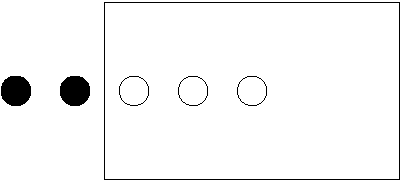
\includegraphics[scale=0.75]{domain-external-staggered}
\end{center}
\caption{A domain (rectangle) with three interior points (empty circles)
and two boundary points (full circles) which are staggered about the
physical boundary.  (This is an exterior boundary.)}
\label{CactusBase:CoordBase:fig-domain-external-staggered}
\end{figure}

\begin{figure}
\begin{center}
\includegraphics[scale=0.75]{domain-internal-staggered}
\end{center}
\caption{A domain (rectangle) with two interior points (empty circles)
and two boundary points (full circles) which are staggered about the
physical boundary.  (This is an interior boundary.)}
\label{CactusBase:CoordBase:fig-domain-internal-staggered}
\end{figure}

Finally, the integer parameter {\texttt{boundary\_shiftout\_x\_lower}}
can be used to shift the boundary points outwards (or inwards with
negative values) by multiples of the grid spacing.  Figure
{\ref{CactusBase:CoordBase:fig-domain-external-shiftout}} shows an
example of an exterior, non-staggered boundary with a shiftout of one.

\begin{figure}
\begin{center}
\includegraphics[scale=0.75]{domain-external-shiftout}
\end{center}
\caption{A domain (rectangle) with four interior points (empty circles)
and two boundary points (full circles) which are shifted outwards by
one grid point.  (This is an exterior, non-staggered boundary.)}
\label{CactusBase:CoordBase:fig-domain-external-shiftout}
\end{figure}

The following table gives examples for common situations:

\begin{tabular}{l|ccc|l}
Boundary condition & internal? & staggered? & shiftout & example \\\hline
reflection symmetry, not staggered & no & no & 1
   & figure {\ref{CactusBase:CoordBase:fig-domain-external-shiftout}} \\
reflection symmetry, staggered & no & yes & 0
   & figure {\ref{CactusBase:CoordBase:fig-domain-external-staggered}} \\
periodicity, closed boundary & no & no & 1
   & figure {\ref{CactusBase:CoordBase:fig-domain-external-shiftout}} \\
periodicity, open boundary & no & no & 0
   & figure {\ref{CactusBase:CoordBase:fig-domain-external}} \\
periodicity, staggered boundary & no & yes & 0
   & figure {\ref{CactusBase:CoordBase:fig-domain-external-staggered}}
\end{tabular}

For other boundary conditions such as Dirichlet or Robin, one can
choose these parameters freely.

\section{Querying about boundary points}
\label{CactusBase:CoordBase:boundary-query}

When iterating over grid points, one usually needs to know about the
boundary sizes and boundary types present. One convenient way is
provided by the aliased function \texttt{GetBoundarySizesAndTypes}:
\begin{verbatim}
CCTK_INT FUNCTION GetBoundarySizesAndTypes
  (CCTK_POINTER_TO_CONST IN cctkGH,
   CCTK_INT IN size,
   CCTK_INT OUT ARRAY bndsize,
   CCTK_INT OUT ARRAY is_ghostbnd,
   CCTK_INT OUT ARRAY is_symbnd,
   CCTK_INT OUT ARRAY is_physbnd)
\end{verbatim}
The input argument \texttt{size} describes the size of the four output
arrays as allocated by the caller, and should be \texttt{2*cctk\_dim}.
The output of this routine describes, for each of the faces of the
domain:
\begin{description}
\item[\texttt{bndsize}] The number of boundary points
\item[\texttt{is\_ghostbnd}] Whether this face is a ghost
  (inter-process) boundary
\item[\texttt{is\_symbnd}] Whether this face is a symmetry boundary
\item[\texttt{is\_physbnd}] Whether this face is a physical boundary
\end{description}

\section{Driver Issues}

When using the CoordBase domain and boundary parameters, the driver
(PUGH, Carpet, etc) also needs to be kept informed.

Whichever driver you're using, if you're specifying the number of boundary
zones using CoordBase, note that this does \textbf{not} automatically
carry over to the \verb|driver::ghost_size_x|, \verb|driver::ghost_size_y|,
and \verb|driver::ghost_size_z| parameters.  If you want the ghost sizes
to be anything other than their defaults (currently~$1$), you need to set
them explicitly.

\subsection{PUGH}

If you're using PUGH, you \textbf{must} still explicitly set the
parameters \verb|driver::global_nx|, \verb|driver::global_ny|,
and \verb|driver::global_nz|.  If you don't set these parameters,
PUGH will assume a default $10 \times 10 \times 10$~grid, which is
almost certainly not what you want!

\subsection{Carpet}

If you're using Carpet, things are nice:  just set
\begin{verbatim}
Carpet::domain_from_coordbase = true
\end{verbatim}
and Carpet will get all its grid information from CoordBase.

% Do not delete next line
% END CACTUS THORNGUIDE

\end{document}
